% This is a sample LaTeX input file.  (Version of 12 August 2004.)
%
% A '%' character causes TeX to ignore all remaining text on the line,
% and is used for comments like this one.

\documentclass{article}      % Specifies the document class

\usepackage{graphicx}		 % Need this to include images
\usepackage[pdfencoding=auto]{hyperref}
\usepackage{amsmath}
\usepackage{amsthm}
\usepackage{xcolor}
\usepackage{algpseudocode}
\usepackage{caption}
\usepackage{subcaption}

%% Define a HUGE 
\makeatletter
\newcommand\HUGE{\@setfontsize\Huge{50}{60}}
\newcommand\todo[1]{\textcolor{blue}{\textbf{todo: }#1}}
\makeatother

\newtheorem{theorem}{Theorem}[section]
\newtheorem{invariant}{Invariant}%[subsection]
\newtheorem{lemma}{Lemma}[section]
\newtheorem{example}{Example}[subsection]

\captionsetup{textfont=it,font=small}

\DeclareMathOperator\mate{\emph{mate}}
\DeclareMathOperator\level{\emph{level}}

\begin{document}             % End of preamble and beginning of text.
%titlepage
\thispagestyle{empty}
\begin{center}
\begin{minipage}{0.9\linewidth}
\flushright
	      		 
	%University logo
    \includegraphics[width=0.5\linewidth]{univie.jpg}\par
    \vspace{1cm}
\centering 	
    % Title
	{\scshape{\HUGE Bachelorarbeit\par}}
	\vspace{1cm}
	%Thesis title
    {\scshape{\Large engineering algorithms for fully dynamic maximal matching\par}}
    \vspace{2cm}
    
  
 Verfasser  \linebreak
 {\Large Richard Paul\par}
 	\vspace{1.5cm}
angestrebter akademischer Grad\linebreak
 {\Large Bachelor of Science (BSc)\par}
	\vspace{1.5cm}

\flushleft
	

\begin{tabular}{ll}
Wien, 2018 \linebreak
\vspace{1cm}&   \\
  Studienkennzahl lt. Studienblatt: & A 033 521 \vspace{0.2cm} \\ 
  Fachrichtung: & Informatik  -  Scientific Computing \vspace{0.2cm} \\
  Betreuerin: & Prof. Dr.Monika Henzinger \vspace{0.2cm} \\
  Co-Betreuer & Dr. Christian Schulz \vspace{0.1cm} \\
  & Shahbaz Khan, PhD
  \end{tabular}


    
    
\end{minipage}
\end{center}
\clearpage

\section*{Acknowledgements}

%\section*{thoughts and comments, to be commented}

%examining runtime behaviour in dependence of n and m is best done by running many experiments with increasing problem size, then compare average update time.

%of most interest is the deletion process. it is fairly easy to maintain a maximal matching when we perform only additions. maintaining a maximal matching when edges disappear is harder since it is naively of complexity O(deg(u)), which can be up to n-1.

%bounding the degree of free vertices therefore is a key task to bound time complexity.


\pagebreak

\begin{abstract}

\end{abstract}

\pagebreak

\tableofcontents

\pagebreak

\section{Introduction}
\label{sec:intro}

\subsection{Motivation}
\label{sec:motivatio}

In graph theory a matching of a graph $G$ is a subgraph $M \subseteq G$ where every vertex has maximally one edge incident to it. Finding an arbitrary matching for a graph is a trivial task, since a single edge already qualifies as a matching. However finding matchings that satisfy more specific properties is not as trivial. \todo{The most common matching problem is the search for maximum cardinality matchings in a graph}. A matching is maximal if it is not a true subset of any other matching, in other words if there exists no edge, which we can add to the matching in order to increase the matchings cardinality without violating the matching condition.

\todo{The calculation of matchings is often needed in combinatorial optimization problems and many real-world application problems, especially from operations research, can be reduced to matching problems.} Calculating maximum matchings in a static graph is a well researched topic with algorithmic solutions developed in the 1960's by Jack Edmonds \todo{cite} and later improvements from Micali and Vaziran in the 1980's \todo{cite}. The graphs derived from the mentioned real-world applications however tend to be dynamic graphs, meaning that over time they undergo changes like loss and creation of new edges. Therefore it has become a relevant topic developing algorithms which try to maintain a maximal matching in a dynamic graph. This problem is called dynamic maximal matching.

The most naive way to solve this dynamic maximal matching problem is to recalculate the matching every time an update on the graph has occured. This however is obviously a wasteful approach regarding the running time. The aim therefore is to find algorithms, that can maintain a maximal matching based on the previously computed matchings and which can compute an update in way less time than the best static algorithm would take.

Traditionally, the development of algorithms is done in a theoretical and very formal manner, resulting in mathematically proofable bounds of complexity. Yet these bounds always take worst-case scenarios into regard, which in real-world applications often do not or only very seldomly occur. A modern approach is known and described as \emph{algorithm engineering} \todo{cite} or \emph{experimental algorithmics} \todo{cite}, which tries to focus more on real-world problems and applications, measuring performance using less formal methods but experimemtal ones. \todo{cite}

\subsection{Contribution and Methods}
\label{sec:cont-meth}

%In this paper we use an algorithm engineering approach to measure performance and quality of three dynamic maximal matching algorithms experimentally using real-world graphs taken from the Koblenz network collection (KONECT) \todo{cite}.

\subsection{Structure}
\label{sec:struct}

This work is structured as follows. After clearifying basic terms and concepts in Section \ref{sec:prelim}, we discuss some related work in Section \ref{sec:rel}. In Section \ref{sec:algorithms} we present the different dynamic algorithms, that we examine throughout this paper. The main part of this paper is in Section \ref{sec:exp-eval} and especially in Section \ref{sec:results}, where we present the results of our experimental evaluation of the previous introduced and discussed algorithms. Our conclusion is presented in Section \ref{sec:conclusion}.

%x preliminaries
%x overview over the algorithms
%experimental evaluation, results
%possible improvements,
%evaluation of improvements 

\pagebreak
\section{Preliminaries}
\label{sec:prelim}

%what is a matching? what is a maximal matching? what is an augmenting path?

\subsection{Matchings}
\label{sec:matchings}

In graph theory a \emph{matching} $M$ of a simple graph $G=(V,E)$ is defined as a subset of edges $M \subseteq E$ where no vertex from $V$ is incident to more than one edge from $M$. In other words, if we construct the graph $G'=(V,M)$, then all vertices in $V$ have either degree $0$ (we call them \emph{free} or \emph{unmatched}) or $1$ (we call them \emph{unfree} or \emph{matched}). For every vertex $u$ with degree of $1$, we call the vertex $v$ at the other end of the incident edge the \emph{mate} of $u$, which we denote as $\mate(u)=v$. For an unmatched vertex $u$ we define $\mate(u)=\bot$. Note that we call an graph without self-loops and without parallel edges a \emph{simple graph}. The \emph{cardinality} or \emph{size} of a matching is simply the cardinality of the edge subset $M$.

An \emph{augmenting path} is defined as a cycle-free path in the graph $G$, that starts and ends on a \emph{free} vertex and where edges from $M$ alternate with edges from $E \setminus M$. The \emph{trivial augmenting path} is a single edge, that has both its endpoints unmatched. If we take an augmenting path and change it by matching every unmatched edge and unmatching every matched edge, we increase the matching cardinality by one.

Further we call a matching \emph{maximal}, if there is no edge in $E$, that we could add to $M$ without corrupting the previously introduced matching condition. We call a matching a \emph{maximum matching}, if it is maximal in size compared to all other valid matchings. The cardinality of a maximum matching is called the \emph{matching number} $\nu(G)$. As proven in \cite{berge57} any maximal matching without \emph{augmenting paths} is a maximum matching. 

We call an $a$-\emph{approximate} maximum matching a matching, that contains at least $\frac{\nu(G)}{a}$ number of edges. Hopcroft and Karp \cite{hopkarp71} showed that any maximal matching with no augmenting paths of length at most $2k-3$ is a $(k/(k-1))$-approximate matching. By setting $2k-3=1 \to k = 2$ we can show that any maximal matching is therefore at least a $2$-approximate maximum matching.

\subsection{Dynamic Graphs and Sequences}
\label{sec:dyn-graphs-seqs}

Unlike the classical maximal matching problem, which tries to compute a matching for static graphs, we focus in this work on \emph{dynamic graphs}, where the number of vertices is fixed, but edges can appear and disappear. The algorithms examined do not recompute the matching for every instance of the graph at a given moment of time $t$, but try to maintain a maximal matching over time. We call a \emph{sequence} $S$ a sequence of edge insertions and deletions. A sequence $S$ of length $k$ is a $k$-tupel of $3$-tupels $(m,u,v)$, where $m$ denotes the input mode ($0$ for deletion, $1$ for insertion), and $u$ and $v$ denote the edge. Note that $G$ is undirected and $(u,v)=(v,u)$ holds. We denote a single sequence step for a given point in time $t$ as $S_t$. 

Furthermore let $\mathcal{G}=\{G_0, G_1,\dots, G_k, G_{k+1}\}$ be a dynamic graph, where $G_i$ denotes the graph constructed from applying the sequence step $S_{i-1}$ on $G_{i-1}$. Note here that $G_0$ is the graph without edges, therefore we obtain $k+1$ static graph instances from a sequence of length $k$. Our definition of dynamic graphs does only consider the edge set to by dynamic, whereas the set of nodes remains the same for all static instances $G_i \in \mathcal{G}$. Therefore we simply write $V$ or $\mathcal{V}$ to denote the node set of the dynamic graph $\mathcal{G}$ as well as every static instance $G_i$. On the other hand the edge set $\mathcal{E}$ of the dynamic graph $\mathcal{G}$ is defined as $\mathcal{E}=\{ E_0, E_1, \dots, E_k, E_{k+1} \} $, where $E_i$ is the edge set of the static graph instance $G_i$. Also let $\mathcal{M}=\{M_0, M_1,\dots, M_i,\dots, M_k, M_{k+1}\}$ be the set of matchings for the according graph $G_i$ for some point in time $t=i$.

According to \todo{[cite http://forskning.diku.dk/PATH05/CRC-book1.pdf]} we can divide dynamic graph problems into three different kinds depending on the kind of updates allowed. A problem where only edge insertions are allowed is called an \emph{incremental} problem, whereas a problem where only edge deletions are allowed is called \emph{decremental}. If both updates are allowed we call the problem \emph{fully dynamic}. In this paper we address the problem of maintaining a maximal matching in a fully dynamic graph. Accordingly all algorithms presented can handle edge insertions as well as edge deletions.

\pagebreak
\section{Related Work}
\label{sec:rel}

\todo{}

\pagebreak
\section{Algorithms}
\label{sec:algorithms}

In this section we give an overview over the implemented and revised fully dynamic algorithms. We begin with the most naive algorithm, which is of complexity $O(n)$. Further we revise a random walk algorithm with different variations, that range from complexity $O(1/\epsilon)$ to $O(n)$ and finally two algorithms by Baswana et al. and Neiman and Solomon. All these algorithms work on fully dynamic graphs and assume that the graph is empty at $t=0$ and that for every sequence step $S_t$ only one insertion or deletion is processed.

\subsection{A Naive Approach}
\label{sec:naive}

In this section we describe a naive algorithm to maintain a maximal matching in a dynamic graph in $O(n)$ time.

\subsubsection{Edge Insertion}
\label{sec:naive-edge-in}

The most naive approach to handle an edge insertion is to check if both endpoints are free and if so add the edge to the matching, otherwise simply ignore it. For a sequence, that consists of insertions only, this approach maintains a maximal matching.

\begin{lemma}
Given the graph $G_i=(V,E)$ and a matching $M_i$, that is maximal with respect to $G_i$, the naive algorithm will maintain a maximal matching $M_{i+1}$ for $G_{i+1}$ when adding an arbitrary edge $(u,v), \, u,v \in V$.
\end{lemma}

\begin{proof}
\todo{}
\end{proof}

\subsubsection{Edge Deletion}
\label{sec:naive-edge-out}

When removing an edge $(u,v)$, we also have to distinguish two cases: An edge, that is to be removed, can either be matched or unmatched. Removing an unmatched edge has neither an effect on the matching size nor does it change the state of an incident vertex, therefore we can simply remove it from the graph. However removing a matched edge does leave the two incident and previously matched vertices free as well as it does decrease the size of the matching by one. These vertices are of special intereset, since, if at least one of them has unmatched neighbours, freeing them has created at least one edge, that could be added to the matching without corrupting the matching condition. Therefore the remaining matching would not be maximal. 

In order to fix this issue, we have to check the surroundings of the freed vertices $u$ and $v$. Checking if there exists a free vertex by scanning through all neighbours of a vertex $w \in {u,v}$ and if applicable match it, is the most simple way to at least assure that our matching remains maximal. This approach takes $O(\deg(u) + \deg(v))$ time, where $\deg(u)$ is the vertex degree of a vertex $u$ and the vertices $u,v$ are the endpoints to the removed edge. The vertex degree in a simple graph is at most $n-1$, where $n=|V|$. Therefore runtime complexity is 
$$
	O(\deg(u) + \deg(v)) = O(n).
$$

\subsubsection{Complexity and Approximation}
\label{sec:naive-complx-approx}

As already mentioned calculating the update for the maintained matching costs $O(1)$ if we handle an edge insertion and $O(n)$ if we handle an edge deletion. \todo{The theoretical notation of $O(n)$ is of course absolutely valid. However especially in the context of application to real-world problems, it is of high interest to keep in mind, that $O(n)$ is in this case derived from the cost of $O(\deg(u) + \deg(v))$. For a dynamic graph $\mathcal{G}$ with an average degree of $\bar{d_{\mathcal{G}}} \ll n_{\mathcal{G}}$ this can have a high impact on the runtime.}

The outlined naive approach maintains a maximal matching in a deterministic way. A maximal matching is known to be a $2$-approximate maximum matching, which means that it contains at least $1/2$ the amount of edges contained in any maximum matching.

\subsection{Random Walk Methods}
\label{sec:random-walk}

As a simple heuristic we extended the naive algorithm by performing random walks whenever an edge is removed in order to detect augmenting paths. We implemented different versions of this random walk algorithm which we will further explain as follows.

Our random walk algorithm handles edge insertions exactly like the naive algorithm does. As shown in the previous Section \ref{sec:naive-edge-in} this approach maintains a maximal matching in $O(1)$ time.

\subsubsection{Edge Deletion and Random Walk}
\label{sec:rw-edge-out}

As mentioned in the naive algorithm, deleting a matched edge $(u,v)$ leaves the two endpoints $u$ and $v$ free. This can give rise to unmatched edges with free endpoints iff there exists a free neighbour for at least one vertex from $\{u,v\}$. If such an unmatched edge exists, that could be added to the matching $M$ after the deletion of $(u,v)$ without conflicting with the matching condition, the matching $M$ is not maximal. We already explained how to maintain the matching maximal in $O(n)$ time. 

If the freed vertices have no free neighbours and the matching before the edge deletion was maximal, then the matching remains maximal. However a free vertex may be starting point to an augmenting path of arbitrary length. Finding such augmenting paths of arbitrary length $k$ in a naive manner costs $O(n^k)$ time and is therefore not a trivial task. In the following we present our random walk approach and four variants which are used as an heuristic approach to find augmenting paths and increase the matching size in order to achieve a better matching quality than the naive algorithm does.

\bigskip \noindent
\textbf{Random Walk:} As an heuristic approach we do a random walk where we assume the walked path to be an augmenting path. We will finish our walk after a maximum of $k=1/\epsilon$ steps latest, where $\epsilon$ is an algorithm parameter. Starting at a free vertex $u$, which at $k=0$ is one of the vertices freed from the deletion of the matched edge, we randomly choose a neighbour $w$ of $u$. If this neighbour is free, then we match the edge $(u,w)$ and our random walk has finished. Otherwise if $w$ is matched, then we unmatch $(w, \mate(w))$ and match $(u,w)$. Note that $u \neq \mate(w)$ since $u$ is free in the beginning and therefore $\mate(u) = \bot$, but $\mate(\mate(w)) = w$ and $w \neq \bot$. Afterwards $\mate(w)$ remains free, therefore we continue our random walk, but starting the next step from $\mate(w)$. Since the decision on where to continue the random walk is done randomly, we do not have to scan anyhow through the neighbours of a vertex. Note that we provide the necessary data structure to retrieve a single neighbour from a vertex in $O(1)$ time. A step in our random walk therefore costs $O(1)$ time, a complete update $O(k) = O(1/\epsilon)$ time.

A closer look at the presented random walk algorithm reveals, that this algorithm cannot guarantee some lower bound for the matching quality. Consider the following scenario. 

\begin{example}
\label{ex:rw-not-max}
There exists a free vertex $x$ which has a neighbour $w$ which is matched with $v$ and which is neighbour of $u$. Our random walk is at its penultimate step, which starts at vertex $u$. Note that the vertices $u,v,w,x$ form an augmenting path of length 3. Our random walk now chooses $v$ randomly from its neighbours. Since $v$ is matched with $w$, we unmatch $(v,w)$ and match $(u,v)$. Our random walk has now performed $k$ steps, it simply breaks out from the recursion. The matching calculated from this update is not maximal, since the two adjacent vertices $w$ and $x$ remain free and the edge $(w,x)$ unmatched.
\end{example}

\noindent
\textbf{max-random-walk:} The presented issue leads us to our first variation of the random walk algorithm. Instead of letting the random walk just suddenly end, we settle the last vertex $z$ naively by scanning through its neighbours for a free vertex. This guarantees, that any matchable edge incident to $z$ will be matched, but takes $O(\deg(z))$ time. As we already examined in Section \ref{sec:naive-edge-out} this is theoretically of cost $O(n)$. %Since this guarantees tat the computed matching is always maximal, we call it \textbf{max-random-walk}.

\bigskip
\noindent
\textbf{$\sqrt{m}$-random-walk:} As a second variant we determined the size of the random walk $k=1/\epsilon$ in dependence of the number of edges present in the graph at time of the update. The maximum length of the random walk is set to $k=\sqrt{m}$, with $m = |E|$. Further this variant does also settle the last node before breaking out from the recursion.

\bigskip
\noindent
\textbf{low-degree-settle:} A third variant checks the degree of every vertex $u$ before continuing its random walk of length $k=1/\epsilon$. If $\deg(u)<1/\epsilon$, then the algorithms tries to settle the vertex naively by scanning through the neighbours of $u$. If settling the vertex was successful, then the we break out from the recursion. Otherwise we keep performing the random walk. The last vertex of our random walk is settled naively as in variant 1, regardless of its degree. 

\bigskip
\noindent
\textbf{extended-naive:} Our fourth variant basically extends the naive algorithm by a conditional random walk. When a matched edge gets removed, the algorithm tries to settle both endpoints naively just as the naive algorithm does. This assures, that the matching remains maximal. However if a vertex remains free after scanning through all its neighbours for a new mate, then it could be the starting point to an augmenting path. Therefore we perform a random walk of length $k = 1/\epsilon$, to possibly detect and augment it. As before, we perform a naive settle at the last step of our random walk in order to guarantee a maximal matching.

\subsubsection{Complexity and Approximation}
\label{sec:rw-complx-approx}

We outlined in the previous section, that our basic variant of the random walk algorithm does not guarantee any particular matching quality. The probability of the described scenario to actually occur is anyhow quite small, wherefore it will be highly interesting, how the algorithm will perform in terms of matching size in the experiments. This lack of a performance guarantee is compensated by the runtime complexity of $O(1/\epsilon)$.

It is the declared goal of our variant 1 of the random walk algorithm to guarantee that our matching remains maximal. As stated previously in Section \ref{sec:prelim} any maximal matching is a $2$-approximate maximum matching. This guarantee happens at cost of runtime complexity, which is increased to $O(1/\epsilon + n)$.

Since the second variant of the random walk algorithm is actually just a differently parametrized variant, that deduces the length of the random walk $k$ from the number of edges $m$ present in the graph as $k=\sqrt{m}$, runtime complexity is $O(\sqrt{m}+n)$. Settling the end vertex of the random walk in a naive manner assures, that our matching is maximal and therefore a $2$-approximate maximum matching.

Querying the degree of a vertex can be accomplished in $O(1)$ time. Performing a naive settle on a vertex is of $O(\deg(u))$ cost. Therefore it costs $O(1/\epsilon)$ time, if we try to perform a naive settle on a vertex during our random walk. Yet if we do not find a vertex during the random walk that we settle, settling the last vertex at the end of the random walk costs $O(n)$ time. Total update time therefore costs $O(n + 1/\epsilon)$ time. We suspect that probability of actually having to perform all $k=1/\epsilon$ steps to be low. Performing naive settle on the last step of our random walk assures, that our matching is maximal after any update.

Since variant 4 is basically the naive algorithm with the extension of performing a conditional random walk, when no mate was found by scanning naively through the neighbours of a vertex $u$, we have runtime complexity $O(n + 1/\epsilon)$. As in the previous variants, we perform a naive settle on the last vertex of the random walk, wherefore this algorithm guarantees the matching to be maximal after any update. Time complexity remains unchanged, since $O(2n + 1/\epsilon) = O(n + 1/\epsilon)$. 

%\todo{This is wrong. When "resolving" an augmenting path there is no guarantee that the (1/eps)-th step does not free a vertex, that has an adjacent free vertex. Therefore it is possible, that an edge exists, that could be added to the new matching, meaning that there is no guarantee for the matching to be maximal. Evaluating this approach experimentally can be anyhow interesting.}

%\subsubsection{Complexity}

% time complexity is mainly determined by maintaining appropriate data structures holding the graph as well as the matching and the parameter epsilon. using a data structure that provides insertion, deletion and access in O(1) time, the runtime complexity for insertion is O(1), for deletion O(1/eps).

\subsection{Randomized algorithm by Baswana, Gupta, Sen}
\label{sec:bgs}

Baswana, Gupta and Sen presented an randomized algorithm in \cite{bgs}, that maintains a $2$-approximate maximal matching in a dynamic graph in \emph{amortized} $O(\sqrt{n})$ time with high probability. This algorithm shows how to improve the runtime of $O(\deg(u)+\deg(v))$ for the earlier mentioned naive approach, where we scan all neighbours of a freed vertex in order to find an appropriate new mate. This improvement is achieved by maintaining a partition of the set of vertices into two disjunct sets and introducing a concept of \emph{ownership} for edges based on this partitioning. 

\subsubsection{Levels and Ownership of Edges}
\label{sec:own-edge}

Baswana, Gupta and Sen partition the set of vertices into two levels 0 and 1. An edge is always owned by at least one of its endpoints. If both endpoints are at level 0, both own the edge. If only one endpoint is at level 1, this endpoint owns the edge. If both endpoints are at level 1, then simply the edge mentioned first will own the edge. A new edge $(u,v)$ with $\mathit{level}(u) = \mathit{level}(v) = 1$ inserted will therefore be owned by the vertex $u$. $\mathcal{O}_u$ denotes the set of edges owned by a vertex $u$. Derived from the partition of the vertices into two levels, Baswana, Gupta and Sen also define the level of an edge $(u,v)$ as $\mathit{level}(u,v)=\max(\mathit{level}(u),\mathit{level}(v))$.

Furthermore the following invariants are introduced:

\begin{invariant}
\label{inv:bgs-1}
Every vertex at level 1 is matched. Every free vertex at level 0 has all its neighbours matched.
\end{invariant}

\begin{invariant}
\label{inv:bgs-2}
Every vertex at level 0 owns less then $\sqrt{n}$ edges at any moment of time.
\end{invariant}

\begin{invariant}
\label{inv:bgs-3}
Both endpoints of every matched edge are at the same level.
\end{invariant}

\subsubsection{Edge Insertion}
\label{sec:bgs-edge-in}

If an edge $(u,v)$ gets inserted and at least one endpoint is at level $1$, the edge can not be naively added to the matching since because of invariant \ref{inv:bgs-1} every vertex at level 1 is matched. In this case, in order to maintain the data structures needed to represent ownership of edges, we add the edge $(u,v)$ to $\mathcal{O}_u$ if $\mathit{level}(u)=1$ or to $\mathcal{O}_v$ if $\mathit{level}(v)=1$. Note, that if both vertices are at level $1$, the edge will be assigned to $u$ only.

Now if no endpoint of an ede $(u,v)$ is at level 1, then the edge will be owned by both endpoints. If both endpoints are free the edge will further be added to the matching. Note that the behaviour of the algorithm matches the behaviour of the naive algorithm so far. The matching maintained is therefore maximal. Adding the edge $(u,v)$ to the sets $\mathcal{O}_u$ and $\mathcal{O}_v$ obviously increases the number of edges owned by $u$ and $v$. This may contradict invariant \ref{inv:bgs-2}. If at least one set $\mathcal{O}_u$ or $\mathcal{O}_v$ exceeds the threshold of $\sqrt{n}$ in size, the vertex $w \in {u,v}$ with the higher number of owned edges will be \emph{repaired}. Repairing a vertex $w$ is done by calling the procedure \textsc{Random-Settle} on $w$. Since $|\mathcal{O}_w|>\sqrt{n}$ the vertex $w$ will be risen to level $1$ at the end of the procedure \textsc{Random-Settle}. Hence we have to remove all edges $(w,x)$, more precisely the vertex $w$, from $\mathcal{O}_x$ for all vertices $x \in \mathcal{O}_u$, since an edge can not be owned by two vertices at level $1$. Note that for any vertex $u$ the set $\mathcal{O}_u$ holds the endpoints for all edges owned by $u$.

\begin{figure}
\center

\begin{algorithmic}[1]
\Procedure{Random-Settle}{$u$}
\State $y \gets \text{randomly chosen element from }\mathcal{O}_u$
\ForAll{$x \in \mathcal{O}_y$}
	\State $\text{remove } y \text{ from } \mathcal{O}_y$
\EndFor
\State $z \gets \textsc{mate}(y)$
\If{$z \neq \textsc{null}$}
	\State $M \gets M \setminus \{(y,z)\}$
\EndIf
\State $M \gets M \cup \{(u,y)\}$
\State $\textsc{level}(u) \gets 1,\,\textsc{level}(y) \gets 1$
\State \Return{$z$}
\EndProcedure
\end{algorithmic}

\caption{Pseudocode for procedure \textsc{Random-Settle}}
\label{pscd:bgs-rs}
\end{figure}

The procedure \textsc{Random-Settle} (see figure \ref{pscd:bgs-rs}) performed on a vertex $u$ picks a mate $y$ for $u$ randomly from the set of owned edges $\mathcal{O}_u$. In order to maintain invariant \ref{inv:bgs-3} $y$ will be risen to level $1$ at the end of the procedure. Therefore we have to do the same we did with $u$ earlier, namely remove the vertex $y$ from $\mathcal{O}_x$ for all vertices $x \in \mathcal{O}_y$. We do so because we stated earlier, that an edge at level $1$ is always owned by only one of its endpoints. Further if $y$ was matched, we unmatch $(y,\mate(y))$, so that we can then match $(u,y)$. Afterwards we set the level of both vertices $u$ and $y$ to $1$. In the end we return the previous mate of $y$. If $y$ was free, we obviously return \textsc{null}.

After performing \textsc{Random-Settle} on $u$, invariant \ref{inv:bgs-2} is reestablished. Note that it suffices to handle only $u$, even when both endpoints of the inserted edge $(u,v)$ own more than $\sqrt{n}$ edges after inserting $(u,v)$. This is because when $u$ rises to level $1$, it takes sole ownership of the edge $(u,v)$. The size of $\mathcal{O}_v$ is therefore reduce by one again and back at its inital size. Naturally the same holds the other way around where only $v$ would be processed.

Furthermore the procedure may leave two vertices free, namely the mate of $u$ from before performing \textsc{Random-Settle} on $u$, if $u$ was matched, as well as the vertex  $z$ returned by the procedure. In order to guarantee, that the matching is maximal, the algorithm tries to settle both vertices $\mate(u)$ and $z$ by scanning through the set of owned edges in search for a free vertex, which can then become the mate of $\mate(u)$ and $z$ respectively. Note the difference to the settle performed by the naive algorithm examined in Section \ref{sec:naive-edge-out}, where we scan through all neighbours.

\subsubsection{Edge Deletion}
\label{sec:bgs-edge-out}

An edge $(u,v)$ can be matched or unmatched when it gets deleted. As we know from the naive algorithm, an unmatched edge being deleted does not affect the matching. For this particular algorithm we can also see, that it does not violate any of the invariants. Note that invariant \ref{inv:bgs-2} does not state, that no vertex at level $1$ is allowed to own less than $\sqrt{n}$ edges.

Obviously no vertex can own the edge $(u,v)$ after it got removed from the graph. It follows that we have to update the according data structures $\mathcal{O}_u$ and $\mathcal{O}_v$ in any case, whether the edges was matched or not. If the edge was not matched, this is the only processing that needs to be done. Otherwise, if the edge was matched, removing it leaves both endpoints $u$ and $v$ free. This might lead to a potential violation of invariant \ref{inv:bgs-1}. 

We distinguish two cases: If the edge was at level $0$, we settle both endpoints $u$ and $v$ naively. Note that because of invariant \ref{inv:bgs-3} we know that $\level(u)=\level(v)$ and therefore can handle both endpoints in the same way. Now if the edge $(u,v)$ was at level $1$, we handle each endpoint $w \in \{u,v\}$ by passing ownership about all edges $(w,x)$ at level $1$ to the respective endpoint $z$. This decreases the size of the set $\mathcal{O}_w$. If the size $|\mathcal{O}_w$ still exceeds or is equal to $\sqrt{n}$, the vertex has to remain at level $1$ because of invariant \ref{inv:bgs-2} and to be settled (according to \ref{inv:bgs-1}). We settle a vertex at level $1$ by performing the earlier introduced routine \textsc{Random-Settle} on it (see figure \ref{pscd:bgs-rs}). As with edge insertion before, the vertex returned by the routine, if it is not \textsc{null}, as well as the previous mate of $w$, if there was one, has to be settled naively. In contrast, if the size $|\mathcal{O}_w|$ is now less than $\sqrt{n}$, the vertex can fall back to level $0$. Since every edge at level $0$ is owned by both its endpoints, we have to add every owned edge $(w,x)$, that is at level $0$, to the set of owned edges of the respective vertex $x$. Afterwards we perform a naive settle on the vertex $w$ to guarantee that invariant \ref{inv:bgs-1} holds. Adding edges to the ownership of $x$ as we did before may increase the size of the set $|\mathcal{O}_x|$ so that it exceeds or is equal to $\sqrt{n}$ and would violate invariant \ref{inv:bgs-2}. Therefore we scan through all owned edges $(w,x)$ and if the size $|\mathcal{O}_x|$ is greater or equal to $\sqrt{n}$, we repair this issue by first performing \textsc{Random-Settle} on the vertex $x$ and then settling the vertex returned by the rountine naively, given that it is not \textsc{null}, and again also the previous mate of the vertex $x$ on which \textsc{Random-Settle} was performed. \todo{We would like to mention, that the particular task of settling the previous mates of $w$ and $x$ is not mentioned in the original paper by Baswana, Gupta and Sen in the section about edge deletion. In order to maintain invariant \ref{inv:bgs-1} it is crucial to do so.}

\subsubsection{Approximation and Complexity}
\label{sec:bgs-approx-complex}

The algorithm proposed by Baswana, Gupta and Sen guarantees that the matching is a $2$-approximate maximal matching after every update. Processing an insertion is done quite similiar to the naive approach, except the processing which is triggered, when a vertex rises to level $1$. In thise case the algorithm is able to detect an augmenting path up to length $5$. This is when the vertex $u$ was matched before we perform \textsc{Random-Settle} on it and further the vertex $z$ returned by the procedure as well as the previous mate of $u$, which has to be free after \textsc{Random-Settle}, are both settled successfully. For an incremental sequence this may increase the quality of the matching over the naive algorithm, however there is no guarantee that this case occurs.

The same case can occur when a matched edge at level $1$ is deleted, falls to level $0$ and thus forces the endpoint of an owned vertex to rise to level $1$, because then \textsc{Random-Settle} has to be performed on this vertex and the previously mentioned scenario can arise. Again, this may lead to an increase of the matching quality in a particular scenario, but does not affect the lower bound on the matching quality.

The fact that the matching is maximal is guaranteed by invariant \ref{inv:bgs-1}. Since no vertex at level $1$ is free, all free vertices have to be at level $0$. Since no vertex at level $0$ has a free neighbour at level $0$, there is no edge that we could add to the matching, that would increase its size. The matching is therefore maximal and a $2$-approximate maximum matching.

\bigskip
\noindent
A key concept of the presented algorithm in order to reduce time complexity is to settle vertices, that have \emph{low} degree using the naive approach and settling those with \emph{high} degree in a randomized manner. In this particular case the threshold between \emph{low} and \emph{high} is $\sqrt{n}$. This approach reduces the costs of settling a vertex naively to $O(\sqrt{n})$. However if we examine the procedure \textsc{Random-Settle}, we can easily see, that it is of cost $O(n)$. In the particular case where an edge at level $1$ is removed, the vertex $u$ on which \textsc{Random-Settle} is performed may own up to $n$ edges. If further none of these edges other endpoints is at level $1$, then we will not remove any edges from the set of edges owned by $u$. The loop in line $3$ in figure \ref{pscd:bgs-rs} will therefore run for $\mathcal{O}_u = n$ times.

Baswana, Gupta and Sen present a sophisticated analysis of their algorithm in order to prove that it achieves \emph{amortized} runtime of $O(\sqrt{n})$. Reproducing their analysis would go beyond the scope of this work. Please refer to their paper \cite{bgs} for detailed examination of the runtime.

\subsection{Deterministic Algorithm by Neiman and Solomon}
\label{sec:ns}

Unlike Baswana, Gupta and Sen in \cite{bgs}, whose algorithm is randomized, Neiman and Solomon \cite{ns} show a deterministic algorithm for maintaining a maximal matching in a dynamic graph. Their approach guarantees, that the matching calculated is a $3/2$-approximate maximal matching and that update time is of $O(\sqrt{m})$ in \emph{worst case}, where $m$ denotes the number of edges present in the graph in the moment of the update.

\subsubsection{Edge insertion}
\label{sec:ns-edge-in}

As mentioned earlier, any matching without augmenting paths of length at most $2k-3$ is a $(k/(k-1))$-approximate maximum matching, meaning that the matching contains at least $(k-1)/k$ fraction of the matching number $\nu(G)$. Remember that the matching number is the size of any maximum matching. Therefore a $3/2$-approximate matching, as Neiman and Solomon guarantee it, is free of any augmenting paths of length at most $3$, which follows from setting $k=3$ for the above equations.

In order to guarantee the approximation of the matching, we have to assure already after each insertion step, that no augmenting path of length $3$ is present. The earlier mentioned, naive approach does only exclude the presence of augmenting paths of length $1$, which is the equivalent to assuring that the matching is maximal. Consider the following example illustrated in figure~\ref{fig:example-4-3-1} for a more detailed explanation.

\begin{figure}
\center 
\includegraphics[width=0.5\textwidth]{example-4-3-1.png}
\caption{Illustration of example \ref{ex:naive-aug-path}}
\label{fig:example-4-3-1}
\end{figure}

\begin{example}
\label{ex:naive-aug-path}
Our dynamic graph $\mathcal{G}$ in this minimal example consists of $\mathcal{V}=\{u,v,w,x\}$ and the dynamic edge set $\mathcal{E}=( E_0 )$ with $E_0=\{\}$ on which we apply the sequence $S = ((1,v,w),(1,u,v),(1,w,x))$. Note that our matching in the beginning is empty, therefore $M_0=\{\}$. Using the naive approach applying $(1,v,w)$ to the graph, where the $1$ signs that we add the edge in this step, results in the matching $M_1=\{(v,w)\}$, since both vertices were free. If we now apply the next two sequence steps, the naive approach will not match any further edges, since for $(1,u,v)$ $v$ is already matched, and for $(1,w,x)$ $w$ is already matched. Therefore the matching after applying the last sequence step is $M_3=\{(v,w)\}$. It is easy to see, that we also have created an augmenting path of length $3$, starting at vertex $u$ and ending on $x$.
\end{example}

\noindent 
Neiman and Solomon address this issue by scanning the surroundings of any edge, that cannot be simply added to the matching for the reason that one endpoint of the edge is already matched. More specifically, if an edge $(u,v)$ cannot be added to the matching, because e.g. $u$ is already matched, we scan the neighbours of the mate of $u$, which we call $u'=\mate(u)$, for a free vertex $x$. By providing appropriate data structures this can be achieved in $O(\sqrt{n})$ time, which we will examine further in Section \ref{sec:ns-complx}. If such a free vertex exists, we have found an augmenting path of length 3, which we augment. This increases the matching size by one. Further an edge insertion, where both endpoints are free, is processed as we already know, namely by simply adding this edge to the matching. Although detecting a vertex as free can be achieved in $O(1)$ time, matching an edge however entails updating several data structures, which takes $O(\sqrt{n+m})$ time as we will explain in a bit (see Section \ref{sec:ns-complx}). An edge with both endpoints matched does not entail any further processing than the one needed to detect them as unfree. Reconsider the earlier example \ref{ex:naive-aug-path}, but this time using Neiman and Solomons approach to update the matching.

\begin{example}
\label{ex:ns-aug-path}
As before let the dynamic graph be $\mathcal{G}=(V,\mathcal{E})=(V,(E_0))=(\{u,v,w,x\},(\{\}))$ and the sequence $S=((1,v,w),(1,u,v),(1,w,x))$. We now apply $S$ on $\mathcal{G}$, where $i$ denotes the step and at each step we apply $S_i$.
\begin{enumerate}
	\item[i=0:] Since for the first step $M_0 = \{\}$ and therefore $v,w \notin M_0$ apply, the first edge $(v,w)$ is added directly to the matching. 	\item[i=1:] In the next step, we add $(u,v)$ to $\mathcal{G}$. Since $v$ is already matched, we check the surroundings of $\mate(v)$ for a free neighbour, however there exists none because the only neighbours of $v$ are $u$, which is $v$'s mate, and $w$, which is the other endpoint of the just added edge. 
	\item[i=2:] In the last step we add $(w,x)$. Again one endpoint is free, namely $x$, and the other one, $w$, is already matched. We scan the surroundings of $v=\mate(w)$ and detect $u$ as free neighbour of $v$. Therefore we have found an augmenting path starting at $x$ and ending at $u$. By inverting the augmenting path we receive the matching $M_3=\{(u,v),(w,x)\}$.
\end{enumerate}
Note that for this particular example the matching $M_3$ is a \emph{perfect} maximum matching. We call a matching \emph{perfect} if there is exists no free vertex.
\end{example}

\subsubsection{Edge Deletion}
\label{sec:ns-edge-out}

As mentioned in Section \ref{sec:naive-edge-out} the process of edge deletion may create new augmenting paths of length $1$, which are simply edges with two free endpoints, but moreover may also create other augmenting paths of arbitrary length. In oder to tackle the augmenting paths of length $1$, the algorithm from Neiman and Solomon checks for both freed vertices whether they have free neighbours and if so matches the freed vertices with those free neighbours. This is done in $O(\sqrt{m})$ time. We examine this improvement in runtime over the naive approach with runtime $O(n)$ more thoroughly in Section \ref{sec:ns-complx}. 

We now focus on guaranteeing that no augmenting paths of length at most $3$ are present in the graph. First we will explain how augmenting paths of length $3$ can rise from an edge deletion using the following example.

\begin{example}
\label{ex:rise-aug-path}
Let $\mathcal{G}$ be a dynamic graph with $\mathcal{V}=\{u,v,w,x,y\}$ and $\mathcal{E}=\{E_0\}$, where $E_0=\{(u,v),(v,w),(w,x),(x,y)\}$ and let $M_0=\{(u,v),(w,x)\}$. Note that this graph and the respective matching can be easily obtained from applying the sequence $ R=((1,u,v),(1,w,x),(1,v,w),(1,x,y)) $ to an empty dynamic graph $\mathcal{G'}=(\mathcal{V},(\{\}))$. 

We now apply a single sequence step $S_0 = (0,u,v))$ to the dynamic graph~$\mathcal{G}$. Removing $(u,v)$ from the graph entails removing the edge also from the matching. This leaves the node $u$ free, but isolated, wherefore it can not be matched again. $v$ at the other hand is then starting point to an augmenting path of length 3, which ends at the free node $y$. Note that the matching $M_1=\{(v,w)\}$ is maximal, but only a 2-approximate to a maximum matching.
\end{example}

\noindent
Neiman and Solomon approach this by checking both freed vertices $u$ and $v$, if they are starting points to augmenting paths. This however does only happen, if the vertex degree is not more than a threshold of $\sqrt{2m}$, where $m$ denotes the amount of edges present in the graph at the moment of the update. For simplicity we will explain the further behaviour of the algorithm for the node $u$, the processing for $v$ is anyhow the same. Finding an augmenting path is done by scanning through all neighbours $w$ of $u$ and checking if $\mate(w)$ has a free neighbour. Naively this would take $O(\min(n,m))$ time, since the runtime complexity of checking all neighbours is dominated by the vertex degree. However as we mentioned previously, this approach is only taken for vertices with a degree less than $\sqrt{2m}$, time complexity is therefore reduced to $O(\sqrt{2m})$. The alternative behaviour will be explained subsequently. Now if an augmenting path has been found, we can invert it in $O(\log n)$ time (see Section \ref{sec:ns-complx}), hence the update time taken from this routine is $O(\sqrt{m})$.

For vertices with degree greater than $\sqrt{2m}$, we find a surrogate $z$ for $u$ with degree of at most $\sqrt{2m}$ who is the mate of a neighbour of $u$. We find such a surrogate by scanning linear through the neighbours of $u$, retrieving $z=\mate(w), w \in N(u)$, where $N(u)$ denotes the set of neighbours of $u$, and then checking if $\deg(z)\leq\sqrt{2m}$. Neiman and Solomon claim, that finding such a surrogate $z$ is done in at most $\sqrt{2m}$ steps, since otherwise the sum of degrees in the graph would be more than $\sqrt{2m} \cdot \sqrt{2m} = 2m$, which is impossible. Now that a surrogate vertex $z$ is found, we unmatch the edge $(w,z)$, match $(u,w)$ and handle $z$ then just as $u$ and $v$ were handled before. Since it is guaranteed, that $\deg{z}<\sqrt{2m}$, an infinite loop can be foreclosed.

We will give another example 

\begin{example}
\todo{todo}
\end{example}

\subsubsection{Approximation}
\label{sec:ns-approx}

As we tried to outline throughout the section, the goal of the algorithm is to maintain a maximal matching that is free from augmenting paths of length at most 3. Following \todo{cite hopcroft and karp} this approach guarantees, that the matching maintained is a $3/2$-approximate maximum matching.

\subsubsection{Complexity}
\label{sec:ns-complx}

In order to bound runtime complexity and guarantee deterministic behaviour, Neiman and Solomon use and maintain the following data structures. 

\begin{itemize}
\item The matching M is saved in an AVL-tree which suppports insertion and deletion in $O(\log n)$ time.
\item For each vertex $x \in \mathcal{V}$ an AVL-tree $N(x)$ is maintained, that holds all neighbours of $x$.
\item A custom data structure $F(x)$ for each vertex $x \in \mathcal{V}$, that contains all free neighbours of $x$ and supports insertion, deletion and querying, if a free neighbour exists, in $O(1)$ time and further allows retrieving a free node in $O(\sqrt{n})$ time.
\item Finally an addressable maximum heap $F_{max}$, which contains all free vetices indexed by their degree. This data structure supports insertion, deletion and updating keys in $O(\log n)$ time, as well retrieving the vertex with highest degree in $O(1)$ time.
\end{itemize}

\noindent
As mentioned earlier, detecting an augmenting path or detecting free vertices can be achieved in $O(\sqrt{n})$ or $O(1)$ time. However matching an edge is not as trivial as it might appear as it does entail updates on the data structure $F(w)$ for all $w \in N(x)$ for all $x \in \{u,v\}$. Naively this would mean update costs of $O(\deg(u) + \deg(v))$ time, which is $O(n)$, since the maximum degree for a vertex in a simple graph is $n-1$, where $n$. In order to bound this update time, Neiman and Solomon introduce two invariants, that state that:

\begin{invariant} 
\label{inv:ns-1}
All free vertices have degree at most $\sqrt{2n + 2m}$.
\end{invariant}

\begin{invariant} 
\label{inv:ns-2}
All vertices, that became free in round $i$ have degree at most $\sqrt{m}$.
\end{invariant}

\noindent
The handling of invariant \ref{inv:ns-2} has been already introduced, but implicitly. The action of finding a surrogate $z$ with $\deg(z)\leq\sqrt{2m}$ for a freed vertex $u$ with $\deg(u)>\sqrt{2m}$, where $u$ remains matched by matching the edge $(u,\mate(z))$, guarantees that any vertex freed in round $i$ has degree not more than $\sqrt{2m}$.

Invariant \ref{inv:ns-1} however has to be handled explicitly by identifying \emph{problematic} vertices, that are \emph{close} to violate Invariant \ref{inv:ns-1}. They call a vertex \emph{problematic}, if it is free and its degree exceeds $\sqrt{2m}$. Neiman and Solomon prove, that it is sufficient to handle one vertex per sequence step additionally to the two vertices, which are already handled by being involved in the performed edge update. This one vertex is the vertex with maximal degree from all free vertices, which can be obtained from the maximum heap $F_{max}$ in $O(\log n)$ time (including removing this vertex from the heap as well as restoring the heap condition). This problematic vertex $x$ is then handled like a vertex $u$ of a freed edge $(u,v)$ with $\deg(u) > \sqrt{2m}$ is handled. This is, we find a surrogate $z$ for $x$, where $z=\mate(y)$, with $y \in N(x)$, unmatch $(z,y)$ in order to be able to match $(x,y)$ and let the surrogate vertex $z$ possibly become free. This however could create new augmenting paths of length $3$ which is why we then call the same procedure, which we use to find augmenting paths from a freed vertex after deletion of a matched edge, to assure that no such augmenting path exists.

\pagebreak
\section{Experimental Evaluation}
\label{sec:exp-eval}

In this section we present how we evaluated the implemented algorithms experimentally and what results we gathered. Our tests were performed on real-world graphs taken from the KONECT database \cite{konect}. Since they provide only few dynamic graphs, we also present methods used to create dynamic sequences of edge insertions and deletions. We evaluate runtime and matching quality of the different algorithms in comparison to each other but also in comparison to the theoretically elaborated upper and lower bounds for runtime and matching quality respectively.

\subsection{Implementation and Environment}
\label{sec:impl-env}

In order to evaluate the previously presented algorithms experimentally, we implemented them in C++11 using g++ version 5.5.0 as compiler. As a base for writing the code we used the KaHIP project \cite{sandersschulz2013}. Unfortunately this project cannot be seen as an extension to KaHIP. The whole code is available at \todo{link to github repo} and is licensed under \todo{some license}.

Our experiments consisted of running different sequences, which will be further described in the following Sections \ref{sec:in-graphs} \& \ref{sec:results}. The sequences were processed by the different algorithms listed in Table \ref{tab:algos} and data about time taken, graph edge cardinality, matching edge cardinality, average vertex degree and average vertex degree of matched vertices was gathered all $r$ steps, where $r$ is a custom parameter. In order to avoid corruption of data, especially the running time, caused by external events on the test machine, every experiment was run several times and the runtime was averaged. Because of the randomized nature of some of the algorithms, we also averaged the matching sizes calculated in each run in order to avoid outliers, which were caused by a particular good or bad seed.

As a benchmark we used GPA algorithm for maximal matching in static graphs to calculate the matchings for the static instances $G_i$ of the dynamic graph $\mathcal{G}$ at the points $i$ in time, where we also gathered the above mentioned data.

Further we also did comparison of all calculated matchings $M_i$, where $i$ is the same point in time $i$ already mentioned. More specifically for a given point in time $i$ we compared all matchings $M_i$ from all algorithms with each other by calculating the intersect of two matchings from two different algorithms. For $l$ algortihms this results in $\frac{l\cdot (l-1)}{2}$ calculated intersects. We did this to better examine the calculated matchings and gather insight to matching similarities.

As a test machine we used a system running Ubuntu 18.04.1 LTS on 4 cores, with 16GB RAM and 100GB disc space. Execution of experiments was done using \texttt{gnu screen} \cite{screen} sessions and also using \texttt{gnu parallel} \cite{parallel} in order to execute several sequential experiments in parallel. This however turned out to be a problem for very big input sequences (about 10M steps), causing memory issues. Regarding the exhaustive use of RAM, we would like to mention, that we could not find any memory leaks using \texttt{valgrind} \cite{valgrind} on our test programs.

\subsection{Input Graphs and Sequences}
\label{sec:inps-seqs}

We present some different approaches used to create fully dynamic sequences from static graphs. Further we give an overview about the real-world graph instances from which we created dynamic sequences in order to run experiments.

\subsubsection{Creating Dynamic Sequences}
\label{sec:dyn-seqs}

We used several graphs from the \emph{Koblenz network collection} (\emph{KONECT}) \cite{konect} as test data. Unfortunately only few of the provided graphs match our requirements of being dynamic, undirected, loop-free and without parallel edges. Since most of the graphs from KONECT are static, we used the following approaches to create dynamic graphs from the static ones provided. 

% Apart from converting KONECT graphs to sequences, that our test program can handle, we can also create sequences from a seed, where the endpoints for an edge, that is to be added are obtained randomly. The limitations in size for the output sequences which are given in the following do not apply to any sequences created from seed. A sequence created from seed is, at least theoretically, not limited in size.

\bigskip \noindent
\textbf{addition-only:} As the name already implies this approach does construct the static input graph by subsequently adding the edges of the static graph to the dynamic one in order of appearance. If the input graph provides time stamps as some of the KONECT graphs do, the edges are first sorted by time stamp and then added. The maximal size of such a sequence is therefore the size of the input sequence. Note that any unprocessed KONECT graph can be seen as a sequence.

\bigskip \noindent
\textbf{random-step:} Before a new sequence step is randomly set to either be an edge insertion or an edge deletion. If it is an edge insertion the next edge in order of appearance or if applicable sorted by time stamps is added to the sequence. Furthermore we maintain an array that contains all edges, that are present in the graph after the recently added sequence step. Hence if the next step is to be an edge deletion, an edge is randomly taken from the array of present edges added as edge deletion to the sequence. Further it gets deleted from the array of edges present in the graph. The maximal size of such a sequence is $2 \cdot l$, where $l$ is the length of the input sequence.

\bigskip \noindent
\textbf{sliding-window:} This approach takes an additional parameter $ws$ to determine the window size of the sliding window. For the first $ws$ sequence steps edges are added in order of appearance or sorted by time stamp. Note that we use $0$-based counting. Afterwards every edge $(u,v)$ added at step $k$ is removed again at step $i=ws+k$. For a input sequence of length $l$, that we convert into a sliding-window sequence, no edges are left to be inserted at step $2 \cdot l - ws$. After this point we continue by deconstructing the graph again by removing edges for the next $ws$ steps as before. The overall maximum length is then $2 \cdot l$ for a given input sequence of length $l$, further the window size $ws$ must not exceed the sequence length $l$.

\bigskip \noindent
\textbf{simple-outage:} As suggested from Bergamini and Meyerhenke \todo{cite} we created sequences, where we remove a randomly chosen edge $(u,v)$ from the graph and then reinsert it in the next step. This approach simulates the outage of a network connection. Similar to the sliding-window method, the first $ws$ sequence steps fill the graph up with edges. In the following phase we continue as already mentioned by removing and reinserting a randomly chosen edge. This method can be used to create arbitrary long sequences, however the window size $ws$ must not exceed the length of the input sequence $l$.

\bigskip \noindent
\textbf{pooled-outage:} As an extension to the simple-outage method this approach does not delete and then reinsert only one edge, but right after the insertion phase creates a pool of size $ps$ by removing $ps$ randomly selected edges. Afterwards we randomly decide for each step whether an edge from the pool is reinserted or another edge is deleted from the graph and therefore added to the pool. The edge cardinality is then expected to be approximately $ws-ps$, where $ws$ is the parameter determining the window size. Like the simple-outage method this approach can be used to create arbitrary long sequences, again the parameter $ws$ must not exceed the length of the input sequence $l$.

\subsubsection{Input Graphs and Parameters}
\label{sec:in-graphs}

\begin{table}
  	\centering
  	\small
  	\begin{tabular}{| l | r | r | c | c |}
    	\hline
    	Name & $n \approx |G|$ & $\approx k$ & Type & Reference \\
    	\hline
%    	amazon & & & \\
		dbpedia & $ 4$M & $ 13.8$M & S & \cite{konect:dbpedia} \\
    	edit-enwiktionary & $ 2.2$M & $ 9$M & T & \cite{konect:editen} \\
    	edit-frwiktionary & $ 1.9$M & $ 7.4$M & T & \cite{konect:editfr} \\
    	facebook-wosn-links & $ 63.7$k & $ 817$k & T & \cite{konect:facebook} \\
    	flickr-growth & $ 2.3$M & $ 33.1$M & T & \cite{konect:flickr} \\
    	link-dynamic-dewiki & $ 2.2$M & $ 86.3$M & D & \cite{konect:dewiki} \\
    	link-dynamic-frwiki & $ 2.2$M & $ 59$M & D & \cite{konect:frwiki} \\
    	link-dynamic-itwiki & $ 1.2$M & $ 34.8$M & D & \cite{konect:itwiki} \\
    	link-dynamic-nlwiki & $ 1$M & $ 20$M & D & \cite{konect:nlwiki} \\
    	link-dynamic-plwiki & $ 1$M & $ 25$M & D & \cite{konect:plwiki} \\
    	link-dynamic-simplewiki & $ 100$k & $ 1.6$M & D & \cite{konect:simplewiki} \\
    	livejournal-groupmemberships & $ 13.9$M & $ 112.3$M & S & \cite{konect:livejournal} \\
    	orkut-groupmemberships & $ 14.3$M & $ 327$M & S & \cite{konect:orkut} \\
    	\hline
    \end{tabular}
  	\caption{Input graphs from KONECT. $k$ denotes the sequence length. For all graphs, except the dynamic ones, $m=|E|=k$ is valid. Regarding the type, S stands for a static graph instance, T for graphs with time stamps and D for real fully dynamic graphs.}
  	\label{tab:graphs}
\end{table}

In table \ref{tab:graphs} we list all graphs that we either used to create dynamic sequences or that already were real dynamic graphs and could therefore be also processed natively.

Because of the earlier mentioned problem of exhaustive memory usage, we could not run our test programs on the full sized instances, but had to truncate them. We did this by creating sequences with up to 250 thousand vertices and about 8 million sequence steps.

The algorithms by Baswana, Gupta and Sen and Neiman and Solomon use thresholds to determine between \emph{low} and \emph{high} degree vertices. In order to test the behaviour of the algorithms for a dense dynamic graph, we also created sequences using the pooled-outage approach with only up to 1000 vertices but 125 thousand vertices. 

\begin{table}
	\centering
	\small
	\begin{tabular}{| l | l | l |}
		\hline
		Algorithm & Abbreviation & $\epsilon$ \\
		\hline
		\hline
		Baswana, Gupta and Sen & bgs & - \\
		Naive & naive & - \\
		Neiman and Solomon & ns & - \\
		Random Walk & $\mathrm{rw}_{0.5}$ & 0.5 \\
		 & $\mathrm{rw}_{0.1}$ & 0.1 \\
		 & $\mathrm{rw}_{0.01}$ & 0.01 \\
		max-random-walk & $\mathrm{mrw}_{0.5}$ & 0.5 \\
		 & $\mathrm{mrw}_{0.1}$ & 0.1 \\
		 & $\mathrm{mrw}_{0.01}$ & 0.01 \\
		$\sqrt{m}$-random-walk & $\mathrm{mrw}_{\sqrt{m}}$ & - \\
		low-degree-settle & $\mathrm{lds}_{0.5}$ & 0.5 \\
		 & $\mathrm{lds}_{0.1}$ & 0.1 \\
		 & $\mathrm{lds}_{0.01}$ & 0.01 \\
		extended-naive & $\mathrm{en}_{0.5}$ & 0.5 \\
		 & $\mathrm{en}_{0.1}$ & 0.1 \\
		 & $\mathrm{en}_{0.01}$ & 0.01 \\
		\hline
	\end{tabular}
	\caption{Algorithms tested during the experiments with parametrization.}
	\label{tab:algos}
\end{table}

The random walk algorithm as well as its variants 1,3 and 4 take a parameter~$\epsilon$ to determine the maximal length of the random walk $k=1/\epsilon$. We tested the random walk algorithm and each of the mentioned variants with the following three different $\epsilon=0.5,0.1,0.01$, which results in maximal length $k=2, 10, 100$ respectively. An overview about all algorithms tested during experiments is given in table \ref{tab:algos}.


%We created from each of the graphs in table \ref{tab:graphs} the 10 sequences seen in \ref{tab:seq-params}. Additionally we ran all real dynamic graphs also as the native sequence they represent. As we mentioned before, we ran into troubles with RAM when processing very large sequences. Hence we truncated the input sequences in length and also in number of vertices, since otherwise it could happen that the graph would become extremly sparse. 

%\begin{table}
%  \centering
%    \begin{tabular}{| l | c | c | c | c |}
%    	\hline
%    	Method & $l$ & $n_{max}$ & $ws$ & $ps$ \\
%    	\hline
%		addition-only & 1000000 & 100000 & - & - \\
%		pooled-outage & 1000000 & 100000 & 100000 & 10\% \\
%		pooled-outage & 1000000 & 100000 & 500000 & 10\% \\
%		pooled-outage & 2000000 & 100000 & 1000000 & 10\% \\
%		pooled-outage & 3000000 & 100000 & 1500000 & 10\% \\
%		pooled-outage & 4000000 & 100000 & 2000000 & 10\% \\
%		pooled-outage & 5000000 & 100000 & 2500000 & 10\% \\
%		random-step & 1000000 & 100000 & - & - \\
%		simple-outage & 1000000 & 100000 & 100000 & - \\
%		sliding-window & 1000000 & 100000 & 100000 & - \\
%    	\hline
%    \end{tabular}
%  	\caption{Parameters used for creating sequences. $l$ denotes the sequence length, $n_{max}$ the maximal vertex ID. $ws$ and $ps$ are window size and pool size as percentage of the window size respectively as introduced in \ref{sec:}.}
%    \label{tab:seq-params}
%\end{table}


\subsection{Results}
\label{sec:results}

In this section we present our results from running the algorithms presented in Section \ref{sec:algorithms} on different sequences. Our main interest lies in the runtime and the matching size achieved by the different algorithms. These graphs were all taken from KONECT \cite{konect}.

\todo{sliding window and simple-outage approaches, summarize results, they are weak because they always do one insertion and one deletion alternately. also the resulting matchings were very similar, which is quite odd, especially regarding the randomized nature of some algorithms.}

\todo {as an improvement we switched to creating sequences using the pooled-outage approach, which is also mentioned in \todo{some papers}. }

\subsubsection{Experiments on Pooled-Outage Sequences}
\label{sec:exp-pool-out}

\begin{table}
	\centering
	\tiny
	\begin{tabular}{| l || r | r | r || r | c || r | c |}
		\hline
		graph & $\approx n_\mathcal{G}$ & 
			$\approx \bar{m}_\mathcal{G}$ & 
			$\approx \mathrm{d}_\mathcal{G}$ & 
			$\approx \max(|\bar{\mathcal{M}}|)$ & by & 
			$\approx \min(\bar{t}_u)$ & by \\
		\hline
		\hline
		dbpedia & $150$k & $ 185.8$k & $ 2.77$ & $ 8777$ & ns & $ 9$ ms & naive \\
		enwikt& $ 142.8$k & $ 305.3$k & $ 4.66$ & $ 3762$ & ns & $ 7.21$ ms & naive \\
		frwikt & $ 149.8$k & $ 318.3$k & $ 4.6$ & $ 606$ & ns & $ 5.83$ ms & naive \\
		facebook & $ 56.1$k & $ 501.2$k & $ 18.46$ & $ 24209$ & mrw$_{\sqrt{m}}$ & $ 11.81$ ms & naive \\
		flickr & $ 42.8$k & $ 463.6$k & $ 23.15$ & $ 1845$ & ns & $ 7.84$ ms & $\mathrm{rw_{0.5}}$ \\
		dewiki  & $ 60.3$k & $ 279.7$k & $ 10.14$ & $ 8090$ & ns & $ 8.38$ ms & naive \\
		frwiki & $ 65.9$k & $ 337.9$k & $ 11$ & $ 15377$ & ns & $ 9.9$ ms & naive \\
		itwiki & $ 71.5$k & $ 367.1$k & $ 10.94$ & $ 17500$ & mrw$_{\sqrt{m}}$ & $ 10.76$ ms & naive \\
		nlwiki  & $ 62.8$k & $ 335.9$k & $ 11.34$ & $ 17581$ & ns & $ 9.81$ ms & naive \\
		plwiki & $ 49.6$k & $ 336$k & $ 14.44$ & $ 13723$ & ns & $ 9.76$ ms & naive \\
		simplewiki & $ 48.9$k & $ 251.7$k & $ 11.02$ & $ 15514$ & ns & $ 9.33$ ms & naive \\
		livejournal & $ 150$k & $ 500.6$k & $ 7.48$ & $ 8276$ & ns & $ 8.62$ ms & naive \\
		orkut & $ 112.7$k & $ 501$k & $ 9.69$ & $ 20059$ & ns & $ 10.19$ ms & naive \\
%		youtube  \\
		\hline
	\end{tabular}
	\caption{Properties and results of pooled-outage sequences. $m_\mathcal{G}$ denotes average amount of edges present throughout the sequence, $\mathrm{d}_\mathcal{G}$ denotes the average degree throughout the sequence.}
    \label{tab:exp-1}
\end{table}

For test set 2, we created pooled-outage sequences from the graphs in Table \ref{tab:graphs} with up to 150k vertices, up to 600k edges present in the graph and approximately 8 million sequence steps. All of these sequences were processed by all algorithms from Table \ref{tab:algos}. As mentioned in Section \ref{sec:in-graphs} the random walk algorithm as well as its variant 1, 3 and 4 were run with three different parameters $\epsilon=0.5,0.1,0.01$. In order to give a general overview we listed detailed properties of the sequences as well as the results from running all algorithms on the according sequence in Table \ref{tab:exp-1}. Further we show the largest average matching size $max(|\bar{M}|)$ achieved and the best average update time $min(\bar{t}_u)$ achieved as well as the corresponding algorithms. In Figure \ref{fig:scatter-150-600} we plotted the distribution of the results computed from the sequences from Table \ref{tab:exp-1}. Every data point in this plot represents the result computed by an algorithm on a particular sequence. 
%Coordinates are computed as the resulting average matching size of the particular result divded by the best average matching size and the best average update time divided by the average update time of the particular result. 
The coordinates $(x,y)$ of a data point in the plot are computed as follows.

Let $i$ be a particular experiment, then
$$
	x = \frac{\min(\bar{t}_{u_i})}{\bar{t}_{u_i}} ,
	\quad\quad
	y = \frac{|\bar{\mathcal{M}_i}|}{\max(|\bar{\mathcal{M}_i}|)} .
$$

The large circles mark the average quality of the respective algorithm, the diameter of the circle represents to the variance of all results computed by the algorithm.

\begin{figure}
	\centering
	\includegraphics[width=\textwidth]{img/exp_150k_600k_scatter.png}
	\caption{Distribution of all experiment results on sequences from table \ref{tab:exp-1}. Matching size and runtime are relative to the respective \emph{best} result, large circle represent average quality and variance of results of the respective algorithm.
	}
	\label{fig:scatter-150-600}
\end{figure}

%that performed best in terms of matching quality and runtimes as well as the respective result achieved by the algorithm. %As one can clearly see, the algorithm by Neiman and Solomon returns averagely the highest matching size. 

%on pooled-outage approach, first experiments resulted in the observation, that the naive algorithm performs best regarding the runtime. this results from the low average degree. 

\bigskip \noindent
As a main result we observed that the naive algorithm outperforms all other algorithms in terms of runtime, as one can easily see in table \ref{tab:exp-1}. This is rather odd since theoretically speaking the naive algorithm has worse runtime complexity than the algorithms by Baswana, Gupta and Sen and Neiman and Solomon. However the more sophisticated algorithms maintain additional data strucutes, which of course takes additional time. The naive algorithm on the other hand is very light-weight in comparison and does not need any additional data structure apart from those needed to store the graph and the matching. %We suspect the phenomena of the very fast naive algorithm to be caused by the small problem size as well as the small average degree of the sequences, since the naive algorithms has expected runtime $O(\bar{d}(G_i))$ at any moment of time $i$.

If we take a look at the average degrees of the sequences, we can see that they are quite low. This may be a cause why the naive algorithm performs so well, since its expected runtime at any point in time $i$ is $O(\mathrm{d}(G_i))$, where $\mathrm{d}(G_i)$ denotes the average vertex degree for the graph $G$. %Note that with our approaches of generating sequences from real-world graph data sets, the vertex degrees in our sequences can not exceed the vertex degrees of the original data set. 
As already mentioned earlier, Baswana, Gupta and Sen and Neiman and Solomon use thresholds to distinguish \emph{low} degree vertices from \emph{high} degree vertices. These thresholds are crucial for the theoretical runtime complexity presented by the authors. The algorithms should perform best in comparison to the naive algorithm when many vertices exceed these thresholds because then $O(\sqrt{m+n}) < O(\mathrm{d}(G_i))$ (for Neiman and Solomon) and $O(\sqrt{n}) < O(\mathrm{d}(G_i))$ (for Baswana, Gupta and Sen) become more likely.

%deduced from this observation we performed further experiments shown in further table with higher average degree. this did not lead to the expected results since still the naive algorithm performed best.

Deduced from this observation we performed further experiments, where we tried to achieve particularly high average vertex degrees. We present the results later in the paper in Section \ref{sec:high-avg-deg}.

\bigskip \noindent
Another interesting observation is the particular bad performance of the basic random walk algorithm with $\epsilon=0.5$ in terms of matching size in Figure \ref{fig:scatter-150-600}. Although the algorithm is the second fastest, the matching size is also the worst among all algorithms. This fact can be explained by the issue, that the matching maintained by the basic random walk algorithm is not maximal, as we already examined in Section \ref{sec:rw-edge-out} and Example \ref{ex:rw-not-max}. We see, that the matching size of the random walk algorithm increases with the length of the random walk $k=1/\epsilon$, however we can also clearly see, that it always performs worse than any of the random walk variants, which guarantee to maintain a maximal matching.

\begin{figure}
	\centering
	\begin{subfigure}[b]{0.25\textwidth}
		\includegraphics[width=\textwidth]{img/graph.png}
		\caption{$|M|=2$}
		\label{fig:rw-aug-a}
	\end{subfigure}
	\qquad
	\begin{subfigure}[b]{0.25\textwidth}
		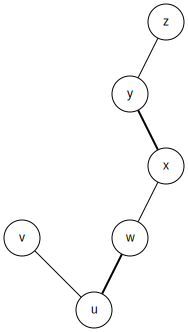
\includegraphics[width=\textwidth]{img/graph2.png}
		\caption{$|M|=2$}
		\label{fig:rw-aug-b}
	\end{subfigure}
	\qquad
	\begin{subfigure}[b]{0.25\textwidth}
		\includegraphics[width=\textwidth]{img/graph3.png}
		\caption{$|M|=3$}
		\label{fig:rw-aug-c}
	\end{subfigure}
	\caption{In \emph{(a)} $u$ was the endpoint of a deleted matched edge, wherefore it remains free right after the edge deletion. In \emph{(b)} we see a possible outcome of random walk variant 1, in \emph{(c)} the outcome of variant 4 for the same scenario. Matched edges are indicated as bold line.}
	\label{fig:rw-augs}
\end{figure}

From the last observation follows also, that the attempt of improving the matching quality made by the random walk variants is quite successful. We can see in the scatter plot \ref{fig:scatter-150-600} that variant 1, which extends the basic random walk algorithm by settling the last vertex naively, does always return a larger average matching size. However variant 4 does return even better results. A random walk performed by variant 1 always carries the risk, that the vertex $u$, on which the random walk was started, could have been settled with some neighbour $v$ but is instead matched with a vertex $w$, that was already matched and was therefore freed. In Figure \ref{fig:rw-aug-a} we illustrated this initial scenario. If the last vertex $z$ of such a random walk remains free, because it has no free neighbour, the matching size remains the same. Further such a random walk creates a new augmenting path starting at its last vertex $z$ and ending at the free neighbour $v$ of the vertex $u$, where the random walk started (see Figure \ref{fig:rw-aug-b}). Variant 4 tries to match the freed vertices of a removed matched edge naively and only if a vertex could not be matched with some new mate, a random walk is performed on that vertex. By doing so, it reduces the number of previously mentioned random walks, that don't increase the matching size and therefore anticipates the creation of the mentioned augmenting path. The result for our illustrated scenario can be seen in Figure \ref{fig:rw-aug-c}. Variant 4 scans through the neighbours of $u$, finds $v$ as a free neighbour and therefore matches the edge $(u,v)$. %\todo{create example plot}

Regarding the particular good runtime of the naive algorithm in Figure \ref{fig:scatter-150-600} we can assume that performing a naive settle is averagely achieved faster than a random walk, at least on the particular test graphs. This explains the runtime improvement of variant 4 over variant 1, since variant 4 performs less random walks than variant 1. 

\todo{why does variant 3 perform as it does? we expected lower running times. we did not actually expect such an improvement in matching quality}

\begin{figure}
	\centering
	\includegraphics[width=\textwidth]{img/exp_150k_600k_eps_quality.png}
	\caption{Matching size results and average matching size from random walk algorithms in dependence of length of the random walk $k$.}
	\label{fig:eps-quality}
\end{figure}

\bigskip \noindent
Although quite expectable we find it noteworthy that increasing the length of the random walks of the different random walk algorithms does result in an improved matching size. This indicates that the declared goal of finding augmenting paths of arbitrary length $l < k$ in order to increase the matching size is quite successful. In Figure \ref{fig:eps-quality} we visualized the matching size and average matching size of the random walk algorithm results as well as the respective~$\epsilon$ used to achieve those results. We expect the matching quality to increase with smaller~$\epsilon$, since a high maximal random walk length does give the chance of finding more augmenting paths. Obviously an arbitrary random walk of length $k$ cannot detect an augmenting path of length $l = k+1$ As we can see with increasing length of the random walk the average matching quality converges asymptotically to the size of the maximum matching.

However this improvement comes at the cost of increased update time per sequence step as we can deduce from Figure \ref{fig:scatter-150-600}. We raise the question, if we can determine some $\epsilon$ experimentally for which further decrement does not improve the matching size significantly. In Section \ref{sec:opt-eps} we peformed further experiments where we ran the random walk algorithms with a variety of different $\epsilon$ in order to answer the raised question.

%\todo{we can generally see that longer random walks indeed increase the matching quality. but we can also see that there seems to be some limit to the improvement because of variant 2 $\to$ find sweet spot in further experiments}

\bigskip \noindent
As stated in Table \ref{tab:exp-1} and observable in Figure \ref{fig:scatter-150-600} the algorithm by Neiman and Solomon does averagely compute the best matching sizes for the given test graphs. This is most probably because of the fact, that it is the only algorithm of the ones we tested, that guarantees that no augmenting path of length at most $3$ exists. Note that all other algorithms do only guarantee the matching to be maximal and therefore to be free of trivial augmenting paths.

\begin{figure}
	\centering
	\includegraphics[width=\textwidth]{img/ns_bgs.png}
	\caption{Average matching size over time for the \emph{dewiki} sequence from Table \ref{tab:exp-1}. Each algorithm was run 5 times, results were averaged. Neiman-Solomon and Baswana-Gupta-Sen are highlighted. \todo{legend missing}}
	\label{fig:ns-bgs-mq}
\end{figure}

In Figure \ref{fig:ns-bgs-mq} we plotted the matching size over time for the experiment on the \emph{dewiki} sequence from in Table \ref{tab:exp-1}. This figure shows a very common result, that we achieved from running our algorithms on the \emph{pooled-outage} sequences described in Section \ref{sec:dyn-graphs-seqs}. For the first $600$k steps we perform only additions, afterwards we start doing insertions and deletions randomly.

A noteworthy phenomena we would like to mention is the gap between the matching size calculated by the Neiman-Solomon algorithm and all other algorithms.% as well as the improvement in matching size that almost all algorithms perform. 
As we already mentioned, the Neiman-Solomon algorithm is the only one to assure the absence of augmenting paths of length at most $3$ and therefore guaranteeing a $3/2$-approximate maximum matching. This obviously has to hold for a pure incremental sequence as well as for a fully dynamic sequence. The gap between the result from the Neiman-Solomon algorithm and the other algorithms indicates that this additional effort does have a significant impact on the matching quality.

In contrary almost all the other algorithms, except Baswana, Gupta and Sen, do handle edge insertions in the naive manner described in Section \ref{sec:naive-edge-in}. This does guarantee us a maximal matching and therefore $2$-approximate maximum cardinality matching in $O(1)$ time. This naive approach works deterministically, which is the reason for the exact similarity of the result of all random walk algorithms as well as the naive algorithm for the pure incremental phase.

By having a look to the close-up in Figure \ref{fig:ns-bgs-mq}, we can see that the result of Baswana, Gupta and Sen does improve slightly over the result of the naive algorithm already during the pure incremental phase. This can be explained by recalling Invariant \ref{inv:bgs-2}, which states, that every vertex at level $0$ owns less then $\sqrt{n}$ edges at any moment of time. Naturally the set of owned edges can increase when new edges are inserted in the graph and therefore also exceed $\sqrt{n}$. If this threshold is exceeded, the algorithm fixes the issue by moving the \emph{dirty} vertex, which violates the invariant, to level $1$, which again is done by performing the routine \textsc{Random-Settle} (see Figure \ref{pscd:bgs-rs}) on it. As we examined in Section \ref{sec:bgs-approx-complex}, calling \textsc{Random-Settle} can detect augmenting paths up to length $3$ and augment them. This results in an increased matching size over the naive insertion process.

\bigskip \noindent
Another observation worth remarking is the sudden change in matching quality for all algorithms except Neiman-Solomon after the pure incremental phase of the \emph{pooled-outage} sequence at about $600$k steps. On the one hand we have the random walk algorithms that perform mainly a steep improvement in the matching size as soon as the sequence starts to contain edge deletions as well as edge insertions. We can observe that the slope increases with smaller~$\epsilon$ and therefore longer maximum random walk length $k=\frac{1}{\epsilon}$. On the other hand we have the naive algorithm as well as the algorithm by Baswana, Gupta and Sen, which improve more slowly, but grow to outperform the random walk algorithms with $\epsilon \geq 0.1$.

Generally, we assume the improvement that sets in when first edge deletions occur to be caused by the fact, that the naive insertion process which is used by these algorithms can create maximal matchings with a high number of augmenting paths. Our assumption is encouraged by the previously mentioned gap between Neiman-Solomon and the other algorithms, which is caused by the exclusion of augmenting paths of length $3$. In such a matching, where no effort has been made to detect and exclude augmenting paths, the number of augmenting paths present in the graph obviously increases. Generally speaking, the deletion of a matched edge can lead to the scenario, where we delete the middle edge of an augmenting path of length $3$. The probability of occurence of such a scenario increases with the number of augmenting paths present in the graph, which is, as we examined, quite \emph{high}. In this case the naive algorithm as well as Baswana-Gupta-Sen and random walk variant 4 do find new mates for the freed endpoints of the deleted edge. This results in an improved matching size of $|M_{i+1}|=|M_i|+1$.

The random walks do have the capability of finding augmenting paths up to length $k=\frac{1}{\epsilon}$, but since they try to detect these augmenting paths in a randomized manner, there is obviously no guarantee, that an augmenting path is found even if there exists one. However the steep slope in matching size of the random walk algorithms does indicate, that the approach of performing random walks does indeed help to find more augmenting paths and therefore to increase the matching size significantly. Further we can also see that more augmenting paths are found with a larger random walk length $k$, which confirms the observations from \ref{fig:eps-quality} addressing the effect of the parameter $\epsilon$ on the resulting mating quality.

We explain the slower increase in matching size for Baswana-Gupta-Sen and the naive algorithm by the fact, that obviously the number $c_{l\geq3}$ of augmenting paths with length $l \geq 3$ is at least as high as the number $c_{l=3}$ of augmenting paths with length exactly $3$, but more probably does exceed $c_{l=3}$ significantly. This alone does not suffice to explain the stronger increase of the random walk algorithms over Baswana-Gupta-Sen and the naive one, since the random walk algorithms do not necessarily have to find such an augmenting path even if there exists one, whereas Baswana-Gupta-Sen and the naive algorithm will find an augmenting path of length 3, if there exists one starting from the respectively handled vertices. However the results of our experiments imply, that the probability of finding an augmenting path of arbitrary length $l \leq k$ with a random walk of maximal length $k$ is at this point indeed higher than the probability, that a matched edge is deleted, which was the middle edge of an augmenting path of length $3$.

As we mentioned, we can see in Figure \ref{fig:ns-bgs-mq} Baswana-Gupta-Sen and the naive algorithm outperform the random walk algorithms with $\epsilon \geq 0.1$ approximately between the sequence steps 2 and 5 million. Throughout this subsequence we have approximately the same amount of edge insertions and deletions. We suspect the reason, that Baswana-Gupta-Sen and the naive algorithm start to outperform the random walk algorithms to lay in the previously mentioned probability of finding augmenting paths of arbitrary length $l \leq k$. By finding augmenting paths and resolving them, we reduce the number of free vertices by two for every augmenting path resolved. This obviously reduces the probability of finding an augmenting path, since there can be maximally $\frac{n_{f,i}}{2}$ augmenting paths being resolved. Note that we use $n_{f,i}$ to denote the number of free vertices in the graph $G_i$. At some point the probability of finding further augmenting paths of length $l \leq k$ using random walks of maximal length $k$ does therefore seem to get so low, that no further improvement in matching size can be observed, although there might still exist free vertices. Although Baswana-Gupta-Sen and the naive algorithm cannot detect augmenting paths of length $l > 3$, the detection of an augmenting path with length 3 of which the middle edge is being deleted is guaranteed, whereas the random walk algorithms can detect such an augmenting path only with probability $\frac{free(u)}{\deg(u)}$. Apparently the probability to find an augmenting path or a free neighbour for a freed vertex randomly is smaller than the probability of deleting such a middle edge of an augmenting path with decreasing $n_f$, which causes the Baswana-Gupta-Sen and naive algorithm to pass the random-walk algorithms with $\epsilon \geq 0.1$.

%This level is naturally reached faster, if averagely more augmenting paths are found per step, since the number of nodes is constant throughout the whole sequence. In contrary Baswana-Gupta-Sen and the naive algorithm do find

%\todo{closer look at neiman solomon and bgs by examining particular test graphs}

%\bigskip
%Notes:
%\begin{itemize}
%
%\item neiman and solomon takes quite long, because of lot of additional data structures but performs constantly well. especially for pure incremental sequences we can clearily see matching quality improvement over the other algorithms caused by the guarantee that there is no augmenting path of length 3.
%
%\item basic random walk algorithm is very fast with big $\epsilon$, the result however has not to be maximal and turns out to be quite bad.
%
%\item random walk variant 1 assures us maximal matching, the matching quality increases noticeable against the basic random walk algorithm, runtime however only slightly increases. this slight increase matches approximately the runtime of the naive algorithm, what matches the expectations.
%
%\item random walk variant 2 takes ridicously long because it takes $O\sqrt{m}$ time. matching quality is quite interesting because it does not increase over the variants with $\epsilon=0.01 \to$  get random walk length which is $\sqrt{m}$
%
%\item %random walk variant 3 runs approximately as fast as variant 1 but with smaller $\epsilon$ the matching quality improves way better. with $\epsilon=0.1$ it outperforms 
%
%\item testing the algorithms with multiple-outage sequences, an interesting phenomena appears. during the incremental addition phase, the neiman-solomon algorithm performs noticeably better than any other algorithm. as soon as the main phase of the sequence starts, where either insertions or deletions can happen with the same probability, the matching computed by the other algorithms start to improve and converge to the solution of the neiman-solomon algorithm. this improvement is differently strong for the different algorithms. for the random walk algorithms we can see, that the length of the random walk has a high impact on this approximation. the reason for this phenomena lays in the fact, that no algorithm except neiman-solomon tries to remove any augmenting paths of length 3 when handling an insertion. however removing the middle edge of an augmenting path of length 3, which is matched, increases the matching size by 1, since both endpoints of the removed edge can be matched again. If no augmenting paths are removed, then the probability that many augmenting paths exist, is quite high. The probability therefore, that the mentioned scenario occurs, increases likewise.
%
%\item can we combine the neiman-solomon approach of guaranteeing that no vertex with deg(u) $> \sqrt{2m+2n}$ is free with the naive approach?
%
%\end{itemize}

\subsubsection{High Average Degree Sequences}
\label{sec:high-avg-deg}

\todo{of any undirected simple graph, the maximal number of edges is $\frac{n(n-1)}{2}$ and the average degree is always some value between $0$ and $(n-1)$. in \cite{bgs} and \cite{ns} the threshold to distinguish between \emph{high} and \emph{low} degree is $\sqrt{n}$ and $\sqrt{2m}$ respectively. to achieve an average degree of $\sqrt{n}$ we need $\frac{n\sqrt{n}}{2}$ edges... }

further experiments with high average degrees did not bring much insight about the running time of the naive algorithm.

\subsubsection{Determining an Optimal $\epsilon$}
\label{sec:opt-eps}

Motivated by the observation that an increased random walk results in an improved matching size, we performed extended experiments on the test sequences from Table \ref{tab:exp-1}. For these experiments, we only ran the random walk algorithms \textbf{max-random-walk}, \textbf{low-degree-settle} and \textbf{extended-naive}, each one parametrized with $\epsilon=0.5, 0.2, 0.1, 0.05, 0.02, 0.01, 0.005, 0.002, 0.001$. 

In Figure \ref{fig:inc-eps-a} we present the results of these experiments. As before in Figure~\ref{fig:eps-quality}, the relative average matching size is the matching size averaged throughout the whole sequence as well as averaged over 5 runs and relative to the best result achieved for the same sequence.

\begin{figure}
	\centering
	\begin{subfigure}[b]{\textwidth}
		\includegraphics[width=\textwidth]{img/diff-eps-1.png}
		\caption{}
		\label{fig:inc-eps-a}
	\end{subfigure}
	\qquad
	\begin{subfigure}[b]{\textwidth}
		\includegraphics[width=\textwidth]{img/diff-eps-2.png}
		\caption{}
		\label{fig:inc-eps-b}
	\end{subfigure}
	\caption{}
	\label{fig:inc-eps}
\end{figure}

The results in Figure \ref{fig:inc-eps-a} match the expectations from the previous experiments. With increasing length of the augmenting path, the matching quality does grow asymptotically against $\nu(\mathcal{G})$ and the improvement does get smaller from step to step. In order to determine up to which point it makes sense to increase the length of the random walk, we define three thresholds $\varphi_0 = 0.001, \varphi_1 = 0.0005, \varphi_2 = 0.0001$, for which we can then examine the relative improvement of matching quality $|\mathcal{M}_k|$ per step $k$:
$$
	\varphi \geq \frac{|\mathcal{M}_{k+1}|}{|\mathcal{M}_k|}.
$$
Note that we use $\varphi$ instead of the $\epsilon$ common in analysis, since  $\epsilon$ is already in use as our random walk algorithm parameter.

In Figure \ref{fig:inc-eps-b} we visualize the relative improvement per step as well as the introduced thresholds $\varphi_0$, $\varphi_1$, $\varphi_2$ and the respective intersections, for which $\varphi = \frac{|\mathcal{M}_{k+1}|}{|\mathcal{M}_k|}$. As we can see, for $\varphi_0$ the relative improvement does fall below the threshold after approximately $k_0=31$, which is $\epsilon_0=\frac{1}{31}\approx0.0323$. For $\varphi_1$ and $\varphi_2$ the respective random walk lengths are approximately $k_1=47$ and $k_2=128$ and therefore $\epsilon_1=\frac{1}{47}\approx0.0213$ and $\epsilon_2=\frac{1}{128}\approx0.0078$.

\todo{examine properties of the test sequences, perform more tests, countercheck the $\epsilon$'s gathered in further experiments}

\subsubsection{Experiments on Real Dynamic Graphs}
\label{sec:exp-real-dyn}

Most of the graphs we used to create test sequences were static or only incremental dynamic graphs, wherefore we used different approaches to create fully dynamic sequences as we presented in Section \ref{sec:dyn-seqs}. In this section we examine the results of our algorithms when ran on real fully dynamic graphs and compare the results with the observations made when running them on the pooled-outage sequences.

The only real fully dynamic graphs found on KONECT are a group of graphs that represent the evolution of hyperlinks between articles on Wikipedia of different languages. As we mentioned in Section \ref{sec:impl-env}, we encountered problems with exhaustive memory consumption, which caused some experiments to fail. As a conclusion, we truncated the real input graphs in order to only process the first 250k vertices and further only the first 8M sequence steps. Unfortunately, for the graphs \emph{itwiki}, \emph{nlwiki} and \emph{plwiki} the experiments still failed, wherefore we focused on the remaining experiments on the graphs \emph{dewiki}, \emph{frwiki} and \emph{simplewiki}.

\begin{table}
	\centering
	\tiny
	\begin{tabular}{| l || r | r | r || r | c || r | c |}
		\hline
		graph & $\approx n_\mathcal{G}$ & 
			$\approx \bar{m}_\mathcal{G}$ & 
			$\approx \mathrm{d}_\mathcal{G}$ & 
			$\approx \max(|\bar{\mathcal{M}}|)$ & by & 
			$\approx \min(\bar{t}_u)$ & by \\
		\hline
		\hline
		dewiki & $250$k & $545.9$k & $7.99$ & $7124$ & ns & $6.03$ ms & rw$_{0.5}$\\
		frwiki & $250$k & $893.6$k & $11.19$ & $20307$ & mrw$_{\sqrt{m}}$ & $ 6.51$ ms & naive \\
		simplewiki & $100.3$k & $362.4$k & $11.38$ & $19279$ & mrw$_{\sqrt{m}}$ & $6.44$ ms & naive \\
		\hline
	\end{tabular}
	\caption{Properties and results of the real dynamic test sequences. $m_\mathcal{G}$ denotes average amount of edges present throughout the sequence, $\mathrm{d}_\mathcal{G}$ denotes the average degree throughout the sequence.}
    \label{tab:exp-real-dyn}
\end{table}

Like the results for the pooled-outage sequences in Table \ref{tab:exp-1} the results in Table \ref{tab:exp-real-dyn} show that the naive algorithm is mostly the fastest one. Unlike the previous results the algorithm \textbf{$\sqrt{m}$-random-walk} does achieve most often the best average matching quality.

\todo{insert figures for real dynamic sequences}

In Figure \ref{fig:dyn-dewiki}, \ref{fig:dyn-frwiki} and \ref{fig:dyn-simplewiki} we plotted the amount of edges present in the graph as well as the matching size throughout the sequence. A main difference between the pooled-outage sequences and all of the real dynamic sequences presented here, lays in the fact that there exists no long and strictly distinguishable incremental phase in the beginning of the real dynamic sequences. Instead edge deletions start to happen already very soon in the sequence. Throughout the whole sequence we have an overall increase of edges, but always also edge deletions. Furthermore we can see peaks in the number of edges after which short subsequences occur, in which edge deletions outweigh.

Regarding the matching size we can see that the gap in the beginning of the sequence between the result of Neiman-Solomon and the other algorithms, that we observed for pooled-outage sequences in Section \ref{sec:exp-pool-out}, is not as noticeably as before. In fact having a closer look at the initial phase, shows a still noticeable improvement of Neiman-Solomon against the other algorithms, however not as distinctive as for the pooled-outage sequences.

This observation can be explained with the phenomena of matching size improvement caused by edge deletions, that we already described in Section \ref{sec:exp-pool-out}. The gap in matching size between Neiman-Solomon and the other matchings results from many \emph{unluckily} matched edges, that cause the creation of augmenting paths of length 3. With increasing length of the pure incremental subsequence, the size of the gap increase, because more and more edges are matched unluckily. As we concluded in Section \ref{sec:exp-pool-out} the edge deletion process of all algorithms except Neiman-Solomon can lead to an improvement of the matching size by detecting and deleting such augmenting paths of length 3. Since for our real dynamic sequences edge insertions and deletions happen in a mixed ratio from the beginning on, such unluckily matched edges may be detected shortly after their creation, which results in a smaller gap between the matching size from Neiman-Solomon and the other algorithms.

\bigskip
\noindent
Another noteworthy difference to the results from Section \ref{sec:exp-pool-out} is the performance of Baswana-Gupta-Sen and the naive algorithm. For the pooled-outage sequences we could observe the matching sizes of Baswana-Gupta-Sen and the naive algorithm grow remarkably and outperform random walk algorithms with $\epsilon \geq 0.1$. This growth is only observable for the results of the \emph{dewiki} sequence in Figure \todo{dewiki matching size}, although less distinctive. Further we cannot observe this kind of growth for the results of the \emph{frwiki} and \emph{simplewiki} sequences. 

Unlike the pooled-outage sequences the real dynamic sequences do not have a long subsequence, where edge insertions and deletions happen almost equally often. Instead we can see from Figures \todo{figures} that overall edge insertions overweigh the deletions. As we stated before, edge insertions do have a probability to create augmenting paths. Therefore it does not come to the situation, where so many augmenting paths have been resolved, that the probability to find further, does grow so small, it hardly occurs and has no more significant effect on growth of the matching size, since new augmenting paths are most probably created throughout the sequence.

As a conclusion to this observation, we consider a subsequence, where edge insertions and deletions happen in an almost equal ratio, as a particular good scenario for the naive algorithm as well as the algorithm from Baswana, Gupta and Sen \cite{bgs}.

\subsubsection{Extending Edge Insertion with Random Walks}

\todo{todo}

\pagebreak
\section{Conclusion}
\label{sec:conclusion}

\pagebreak

\bibliographystyle{acm}
\bibliography{BSc_Latex_Template}

\end{document}
% End of document.